\section{Motivation}\label{sec:motivation}

\begin{figure}[ht]
 \centering
  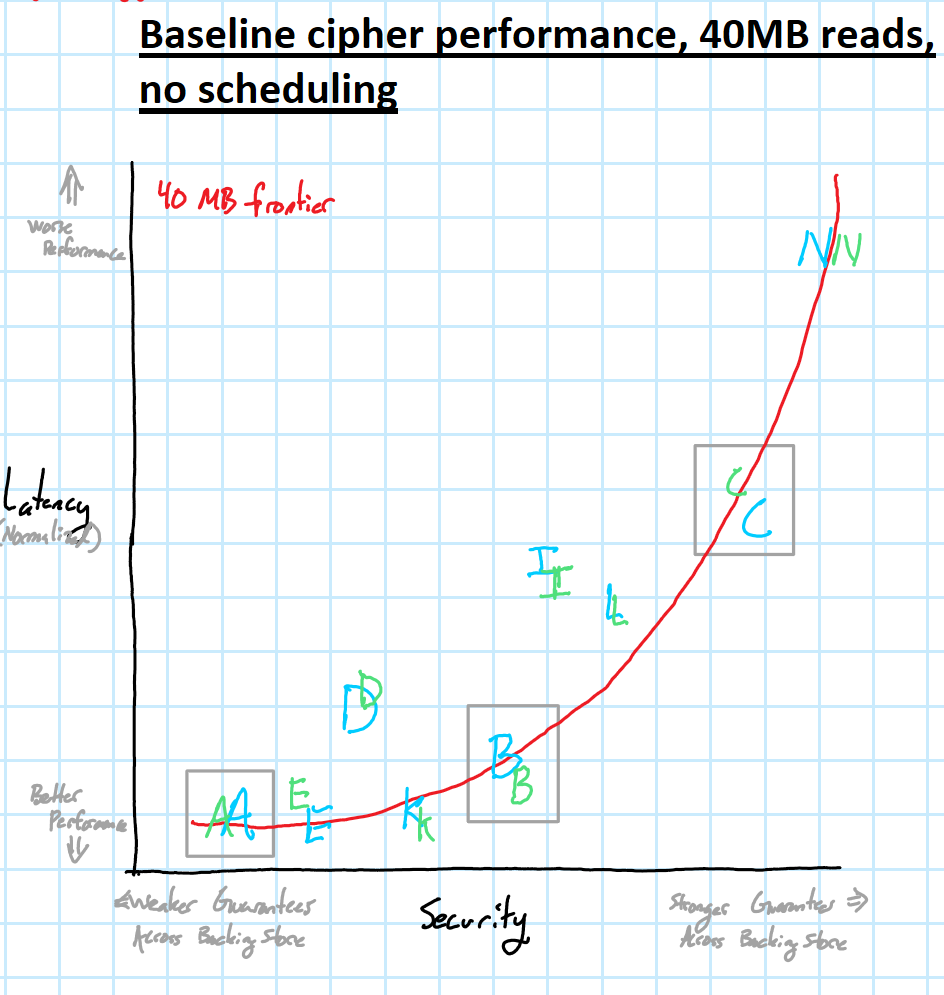
\includegraphics[width=0.8\linewidth]{drawn/1.png}
   \caption{\TODO{Caption goes here}}\label{fig:40mb-read-frontier}
\end{figure}

\figref{fig:40mb-read-frontier}

\begin{figure}[ht]
   \centering
    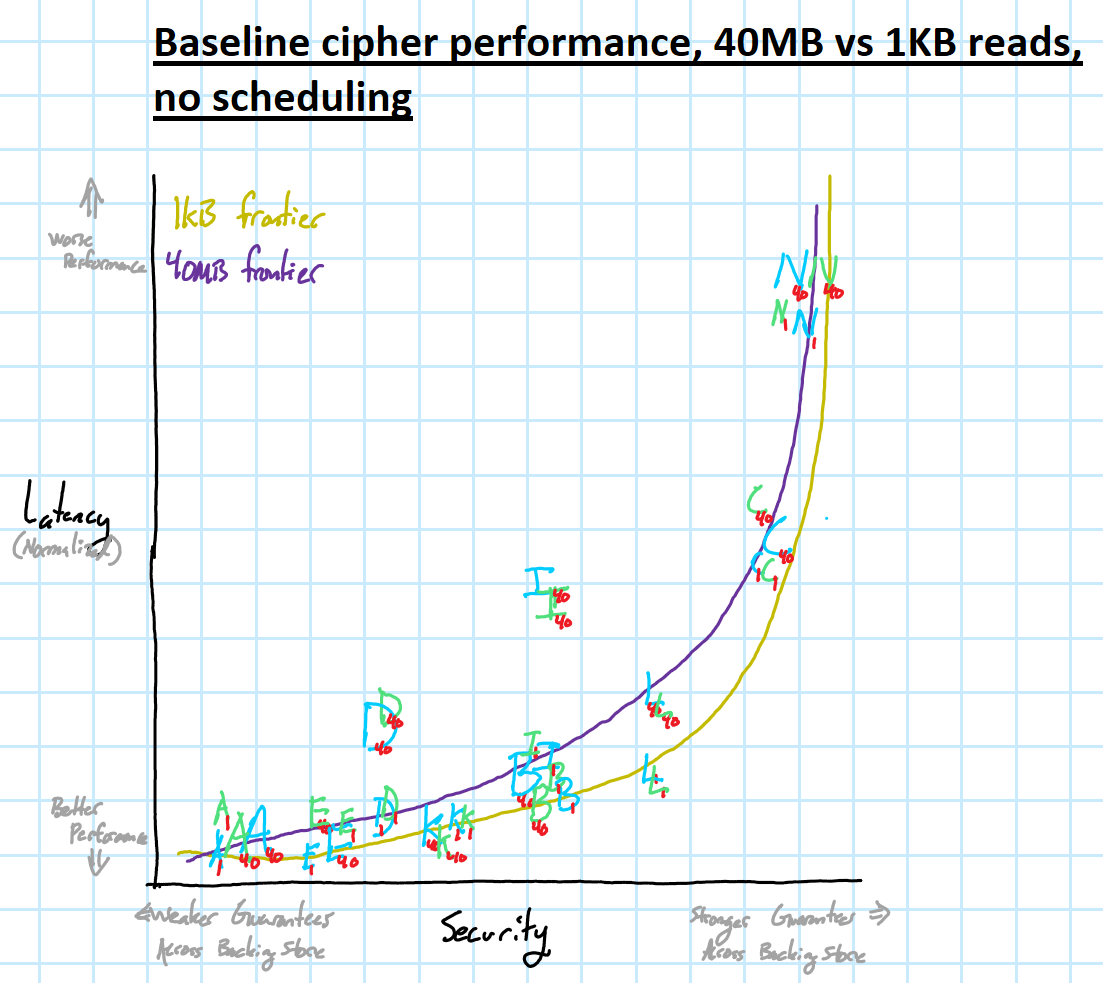
\includegraphics[width=0.8\linewidth]{drawn/2.png}
     \caption{\TODO{Caption goes here}}\label{fig:40mb-1kb-read-frontier}
  \end{figure}

\begin{figure}[ht]
 \centering
  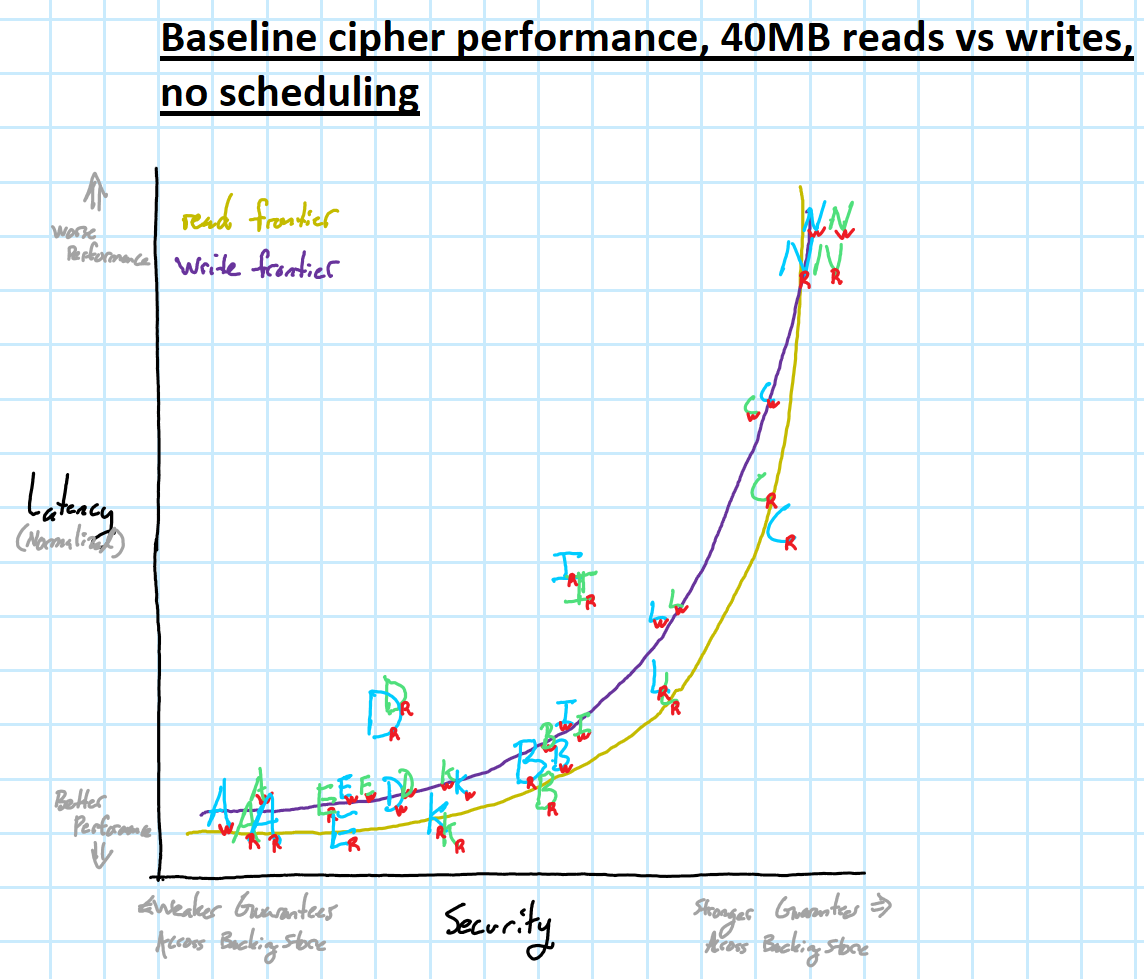
\includegraphics[width=0.8\linewidth]{drawn/3.png}
   \caption{\TODO{Caption goes here}}\label{fig:40mb-read-write-frontier}
\end{figure}

Prior work leveraging Log-structured File System (LFS) behavior to enable the
use of stream ciphers for FDE naturally lends itself to transitioning encrypted
data between different ciphers during runtime. This is because 1) encryption and
decryption of nuggets occurs independently of one another and 2) LFS
"append-mostly" behavior avoids overwrites by ensuring all write operations
target "empty" (\ie{initialized with random data}) space on the backing store.
